\documentclass[a4paper, 11pt]{article}
\usepackage[utf8]{inputenc} 
\usepackage[T1]{fontenc}
\usepackage{lmodern}
\usepackage{graphicx}
\usepackage[french]{babel}
\usepackage[citestyle=authortitle,defernumbers=true]{biblatex}
\addbibresource{bibliographie.bib}
\nocite{*}

\author{Torrenté Florian}
\title{Travail de maturité - Puissance4IA}

\begin{document}
\maketitle

\tableofcontents

\newpage
\section{Introduction}

\subsection{Description et règles du jeu}
    Le Puissance 4 est un jeu avec des règles très simples. Le but du jeu est d'aligner quatre pions de même couleur (horizontalement, verticalement, ou en diagonale). Le terrain de jeu est une grille de 7x6 (sept colonnes et six rangées). Chaque joueur possède les pions d'une couleur (généralement jaune et rouge). Chacun son tour, les joueurs déposent un pion dans la colonne de leur choix, le pion descend alors le plus bas possible dans la colonne. Le premier joueur à aligner quatre pions de sa couleur gagne. S'il n'y a plus de place pour jouer, la partie est nulle.

    \begin{figure}[h]
        \centering
        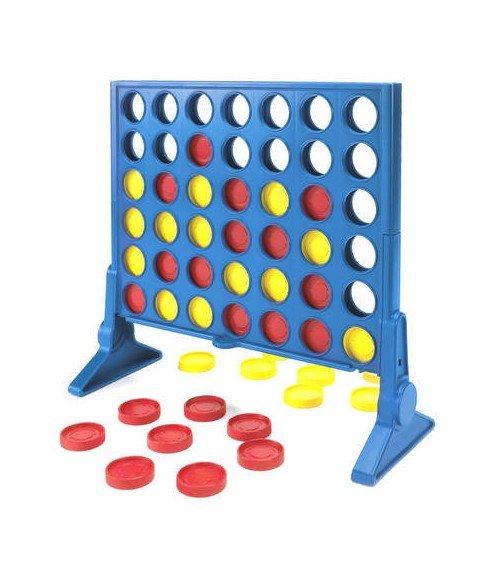
\includegraphics[width=0.5\textwidth]{puissance4.jpg}
        \caption{Un exemple de partie gagnée par le joueur rouge.}    
    \end{figure}

\subsection{L'intelligence artificielle}
    L'humanité s'est donné le nom scientifique \textbf{homo sapiens}---l'homme sage---parce que nos capacités mentales sont extrêmement importantes pour nous et notre sentiment d'identité. Le domaine de l'intelligence artificielle (ou IA) tente de comprendre cette intelligence. C'est pourquoi l'étudier peut nous permettre d'en apprendre davantage sur nous-même. Contrairement à la philosophie et à la psychologie, qui s'intéressent aussi à l'intelligence, l'IA essaye de \textit{construire} des entités intelligentes et de les comprendre. Une autre raison d'étudier l'IA est que ces entités construites sont intéressantes et utiles en elles-mêmes. En effet, ces dernières ont donné naissance à de nombreux résultats significatifs et impressionnants.

    Maintenant nous savons pourquoi l'IA est intéressant et important, nous avons toujours besoin de savoir précisément \textit{ce que c'est}. On pourrait simplement dire: "Eh bien, ça a à voir avec les programmes intelligents", mais je pense qu'il est important bien définir des objectifs pour pouvoir les atteindre. Une définition plus cohérente pour moi serait celle-ci: "L’intelligence artificielle a pour objectif de construire des dispositifs simulant les processus cognitifs humains"\footcite{haiech_2020}
\subsection{Objectifs}

\section{Déroulement du travail}

\subsection{Mise en place}

\subsection{Implémentation du Puissance 4}

\subsection{Implémentation de l'algorithme Minimax}

\subsection{Améliorations de l'algorithme}

\subsection{Tests grandeur nature}

\section{Conclusion}
\subsection{Atteinte des objectifs}
\subsection{Ouverture vers le futur}
\subsection{Remerciements}

\newpage
\section{Bibliographie}
\subsection{Livres}
\printbibliography[heading=none, type=book]
\subsection{Sites web}
\printbibliography[heading=none, type=misc]

\section{Annexes}

\end{document}